% ~~~~~~~~~~~~~~~~~~~~~~~~~~~~~~~~~~~~~~~~~~~~~~~~~~~~~~~~~~~~~~~~~~~~~~~~~~~~~
%
% ULL_thesis_template.tex
%
% A template for creating ULL theses which are compliant with the current
% formatting guidelines published by the Grad School.
%
% Created by: 07/17/17 - Forrest Montgomery 
%
% Modified:
%	* 04/04/18 - Daniel Newman -- danielnewman09@gmail.com
%		- Made this template compliant with Fall 2017 Graduate school guidelines
% ~~~~~~~~~~~~~~~~~~~~~~~~~~~~~~~~~~~~~~~~~~~~~~~~~~~~~~~~~~~~~~~~~~~~~~~~~~~~~
\documentclass[12pt,normalmargins]{gatech-thesis}
\usepackage{amsmath,amssymb,latexsym,float,epsfig}
\usepackage{subcaption}
\usepackage{booktabs}
\usepackage{mathtools,breqn,amsmath}
\usepackage{amssymb}
\usepackage{cite}
\usepackage{bm}
\usepackage{tikz}
\usepackage{titlesec}
\usepackage{tocloft}
\usepackage{indentfirst}
\usepackage{etoolbox}
\definecolor{1c1}{RGB}{188,162,6}
\usepackage{ULL-style}
\usepackage[shortcuts]{extdash}

%%%%%%%%%%%%%%%%%%%%%%%%%%%%%%%%%%%
% Personal Shortcuts
% You will need to type these as \cspm{}
%%%%%%%%%%%%%%%%%%%%%%%%%%%%%%%%%%%
\newcommand{\cspm}{\textsc{cspm}}
\newcommand{\cdpm}{\textsc{cdpm}}
\newcommand{\etal}{\emph{et al.}}
%%%%%%%%%%%%%%%%%%%%%%%%%%%%%%%%%%%


%%%%%%%%%%%%%%%%
% Preliminary Info
%%%%%%%%%%%%%%%%
\title{Design and Control of a \LaTeX{} Thesis Template} 
\author{Forrest Montgomery}
\lastnamefirstname{Montgomery, Forrest}

% ex: {Name}[Position] use \\ if you need a newline
\committeechair{Joshua E. Vaughan}[Assistant Professor of Mechanical Engineering]
\firstreader{Paul Darby}[Assistant Professor of Electrical \\Engineering]
\secondreader{Charles E. Taylor}[Assistant Professor of Mechanical Engineering]
\deanofgradschool{Mary Farmer-Kaiser}[Dean of the Graduate School]

\major{Mechanical Engineering}
\degree{Masters of Science}
\undergrad{Bachelor of Science}
\undergraduniversity{University of Louisiana at Lafayette}
\undergradyear{Spring 2015}

% Must be less than 300
\wordsinabstract{185}

% Total number of pages including the title page.
\totalpagesinthesis{125}
\copyrightyear{2017}

% When you graduate ex: Summer 2017
\submitdate{Summer 2017}

% \bibfiles{example-thesis}
\bibfiles{library}

\begin{document}
\iraggedright

% Change this if you want another bib style.
\bibliographystyle{gatech-thesis}
%%
\begin{preliminary}

%%%%%%%%%%%%%%%%
% Dedication -- (optional)
%%%%%%%%%%%%%%%%

\begin{dedication}
To all the poor souls using Word, one day you will see the light.
\end{dedication}

%%%%%%%%%%%%%%%%
% Epigraph -- A short quote suggesting the theme of the thesis,
% or something random. This is optional.
%%%%%%%%%%%%%%%%

%!TEX root = ULL_thesis_template.tex 
\begin{epigraph}

% An epigraph is a motto or quotation that captures the spirit or meaning of your work
\vspace*{-0.25in}
\begin{center}
% \vspace{-0.25in}
\vspace*{\fill}
% ``If you optimize everything, you will always be unhappy.''\\
% And the worst flaw is that we’re just plain dumb.\\
% Admit it!''\\
% --- Donald Knuth

% \textit{``Research is what I'm doing when I don't know what I'm doing.''}
% \\
% --- Wernher von Braun
\textit{``We can lick gravity, but sometimes the paperwork is overwhelming.''}
\\
--- Wernher von Braun
\vspace*{\fill}
\end{center}

\end{epigraph}

%%%%%%%%%%%%%%%%
% Acknowledgements
%%%%%%%%%%%%%%%%

%!TEX root = ULL_thesis_template.tex 
\begin{acknowledgements}

Lorem ipsum dolor sit amet, consectetur adipiscing elit. Vivamus nec tellus eget elit aliquet accumsan sit amet in lacus. In hac habitasse platea dictumst. Ut sit amet elit odio. Aenean lobortis mollis metus, sed consequat neque tristique in. Curabitur nec hendrerit metus. Praesent non scelerisque urna, vitae iaculis diam. Aliquam nisl est, imperdiet eu nulla sed, bibendum pulvinar arcu. In ultricies purus purus, vulputate congue justo volutpat ut. Donec nunc magna, rutrum nec turpis et, viverra efficitur lorem. In hac habitasse platea dictumst. Vestibulum maximus lobortis nisl, eget molestie sem sollicitudin nec. Mauris ut enim eu ipsum auctor rhoncus ac vel eros.

Vivamus tincidunt, tortor eu rutrum dapibus, orci turpis porta metus, ac iaculis quam eros sollicitudin nisl. Nam id massa elementum, commodo mi at, lobortis nisl. Fusce vestibulum eu lorem non aliquam. Morbi eleifend tortor id metus elementum, ac tincidunt lorem commodo. Pellentesque vestibulum, erat in tempus vehicula, ex urna auctor leo, ut lobortis eros mauris nec erat. Aliquam erat volutpat. Sed sed pretium risus.

Proin vel libero eleifend, convallis nunc eu, sollicitudin elit. Aenean non malesuada ipsum. Vestibulum viverra ullamcorper nibh, vel ornare metus. Nunc quis leo eget ex sollicitudin convallis nec eget tortor. In ipsum turpis, pulvinar ut ligula hendrerit, mollis fermentum dui. Mauris augue elit, scelerisque sit amet scelerisque ac, malesuada ac ligula. Vivamus ac ligula ut risus tincidunt hendrerit.

\end{acknowledgements}

%%%%%%%%%%%%%%%%
% Table of Contents, LOF, and LOT
%%%%%%%%%%%%%%%%
\contents
\end{preliminary}

%%%%%%%%%%%%%%%%
% Chapter 1
%%%%%%%%%%%%%%%%

%!TEX root = ULL_thesis_template.tex 
\chapter{Introduction and Background}
\label{intro}
Lorem ipsum dolor sit amet, consectetur adipiscing elit. Vivamus nec tellus eget elit aliquet accumsan sit amet in lacus. In hac habitasse platea dictumst. Ut sit amet elit odio. Aenean lobortis mollis metus, sed consequat neque tristique in. Curabitur nec hendrerit metus. 

\begin{figure}[b!]
\centering
  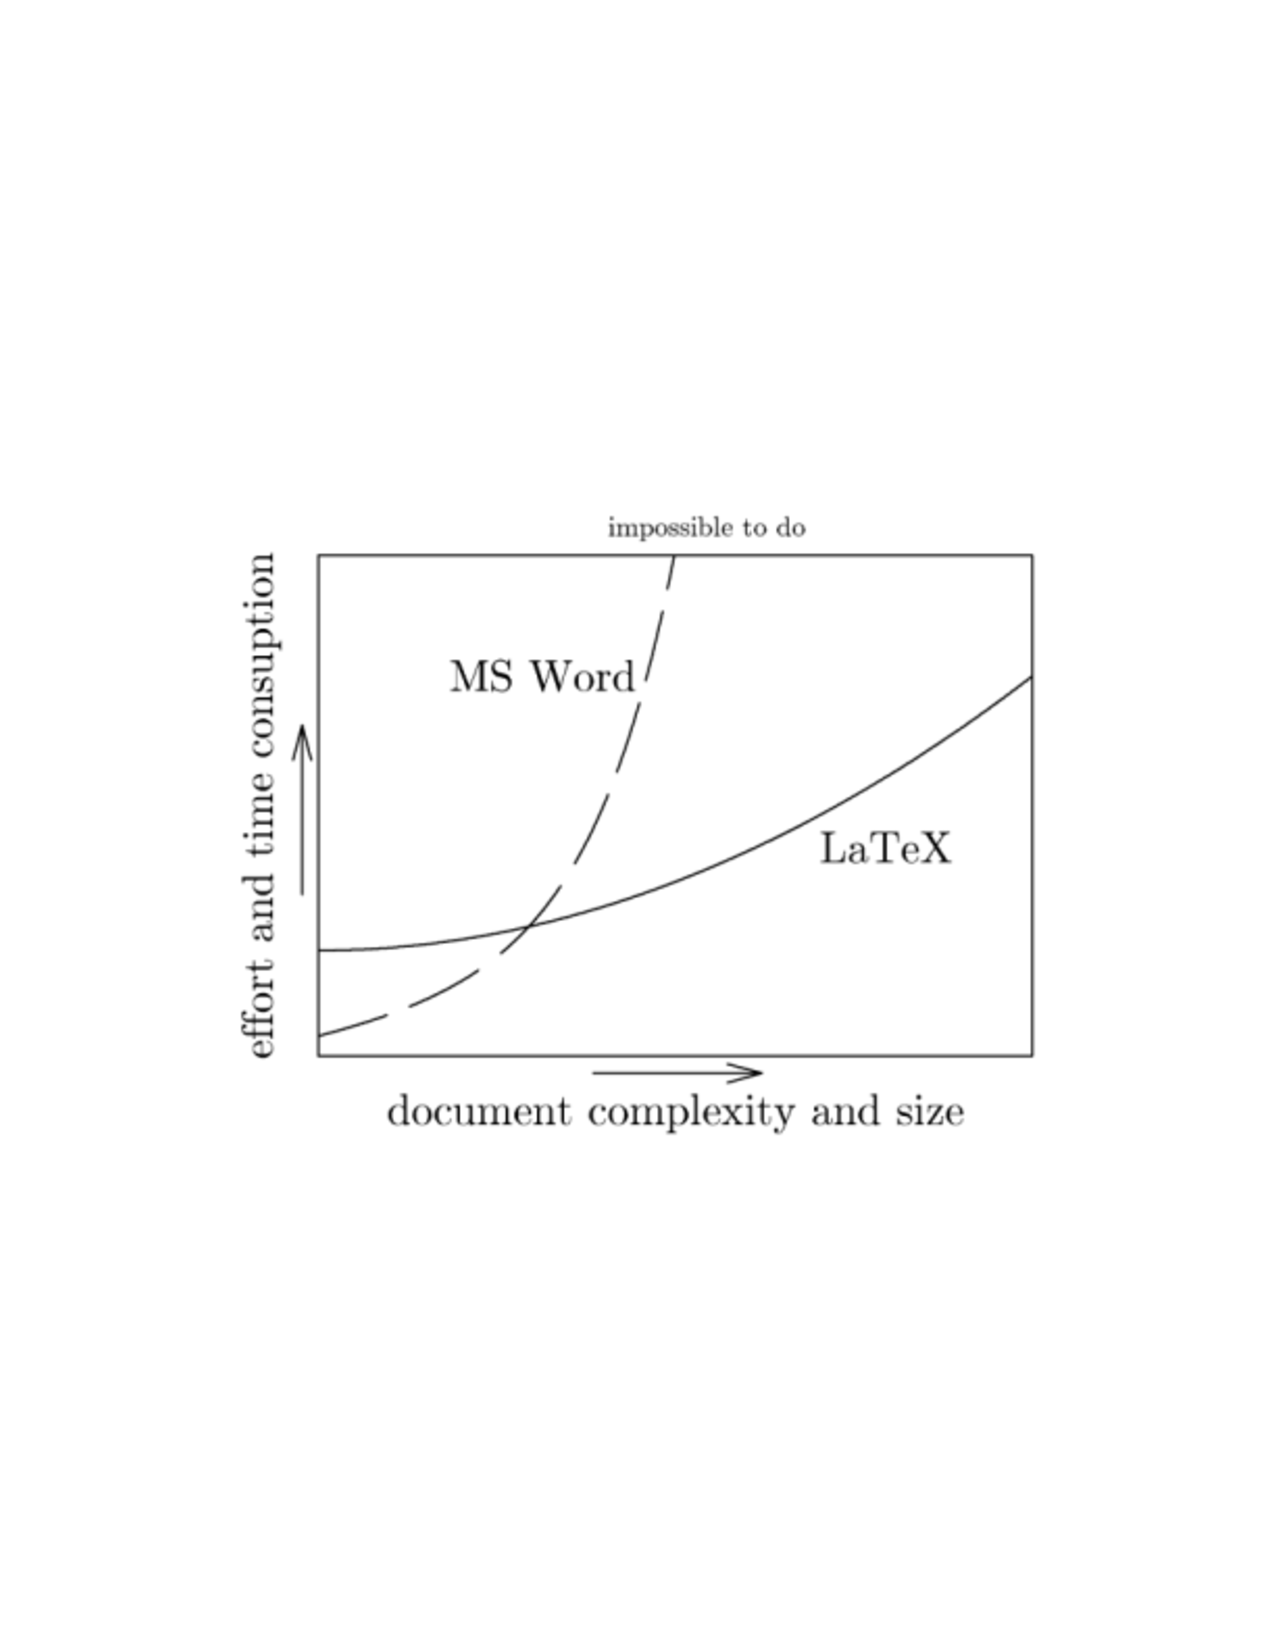
\includegraphics[width=0.5\textwidth]{Figures/Latex.pdf}
  \caption{From Marko Pinteric}
  \label{fig:Latex}
\end{figure}

Praesent non scelerisque urna, vitae iaculis diam. Aliquam nisl est, imperdiet eu nulla sed, bibendum pulvinar arcu. In ultricies purus purus, vulputate congue justo volutpat ut. Donec nunc magna, rutrum nec turpis \ref{fig:Latex} et, viverra efficitur lorem. In hac habitasse platea dictumst. Vestibulum maximus lobortis nisl, eget molestie sem sollicitudin nec. Mauris ut enim eu ipsum auctor rhoncus ac vel eros.

\section{Section}
Vivamus tincidunt, tortor eu rutrum dapibus, orci turpis porta metus, ac iaculis quam eros sollicitudin nisl. Nam id massa elementum, commodo mi at, lobortis nisl. Fusce vestibulum eu lorem non aliquam. Morbi eleifend tortor id metus elementum, ac tincidunt lorem commodo. Pellentesque vestibulum, erat in tempus vehicula, ex urna auctor leo, ut lobortis eros mauris nec erat. Aliquam erat volutpat.

\subsection{Subsection}
Proin vel libero eleifend, convallis nunc eu, sollicitudin elit. Aenean non malesuada ipsum. Vestibulum viverra ullamcorper nibh, vel ornare metus. Nunc quis leo eget ex sollicitudin convallis nec \cite{Maeda1999} eget tortor. In ipsum turpis, pulvinar ut ligula hendrerit, mollis fermentum dui. Mauris augue elit, scelerisque sit amet scelerisque ac, malesuada ac ligula. Vivamus ac ligula ut risus tincidunt hendrerit.

Pellentesque eget accumsan mi. Sed rutrum turpis quis dapibus eleifend. Ut ac ex ullamcorper, pellentesque orci ac, facilisis urna. Phasellus at placerat arcu. Maecenas eu pretium lacus, quis pretium dui. Vestibulum sit amet erat dignissim, suscipit lectus a, malesuada eros. Nullam pellentesque gravida odio, in elementum est bibendum vel. Pellentesque habitant morbi tristique senectus et netus et malesuada fames ac turpis egestas. Mauris in leo rutrum, maximus nisl non, ultricies diam. Donec dictum orci vitae ante efficitur tincidunt id non urna. Lorem ipsum dolor sit amet, consectetur adipiscing elit. Nullam a ipsum ipsum.

\begin{table}[t!]
\centering
\caption{Impulse Amplitudes and Spacing for Two Input Shaper}
\label{table:multi-impulses}
\begin{tabular}{@{}rrrr@{}}
\toprule
\multicolumn{1}{l}{} &  & \multicolumn{2}{c}{Impulse Amplitudes} \\ \midrule
Impulse Times &  & Input $f_1$ & Input $f_2$ \\ \cmidrule(l){3-4} 
0 &  & 0.50 & 0.07 \\
0.84 &  & 0.09 & 0.94 \\
1.69 &  & 0.41 & 0.00 \\ \bottomrule
\end{tabular}
\end{table}
%%%%%%%%%%%%%%%%
% Chapter 2
%%%%%%%%%%%%%%%%

\chapter{Dynamic Model}
\label{chapter2}

Lorem ipsum dolor sit amet, consectetur adipiscing elit. Vivamus nec tellus eget elit aliquet accumsan sit amet in lacus. In hac habitasse platea dictumst. Ut sit amet elit odio. Aenean lobortis mollis metus, sed consequat neque tristique in. Curabitur nec hendrerit metus. Praesent non scelerisque urna, vitae iaculis diam. Aliquam nisl est, imperdiet eu nulla sed, bibendum pulvinar arcu. In ultricies purus purus, vulputate congue justo volutpat ut. Donec nunc magna, rutrum nec turpis et, viverra efficitur lorem. In hac habitasse platea dictumst. Vestibulum maximus lobortis nisl, eget molestie sem sollicitudin nec. Mauris ut enim eu ipsum auctor rhoncus ac vel eros.

\section{Section}
Vivamus tincidunt, tortor eu rutrum dapibus, orci turpis porta metus, ac iaculis quam eros sollicitudin nisl. Nam id massa elementum, commodo mi at, lobortis nisl. Fusce vestibulum eu lorem non aliquam. Morbi eleifend tortor id metus elementum, ac tincidunt lorem commodo. Pellentesque vestibulum, erat in tempus vehicula, ex urna auctor leo, ut lobortis eros mauris nec erat. Aliquam erat volutpat. Sed sed pretium risus.

\subsection{Subsection}
Proin vel libero eleifend, convallis nunc eu, sollicitudin elit. Aenean non malesuada ipsum. Vestibulum viverra ullamcorper nibh, vel ornare metus. Nunc quis leo eget ex sollicitudin convallis nec Well never have I ever \cite{Latexslow} eget tortor. In ipsum turpis, pulvinar ut ligula hendrerit, mollis fermentum dui. Mauris augue elit, scelerisque sit amet scelerisque ac, malesuada ac ligula. Vivamus ac ligula ut risus tincidunt hendrerit.

Pellentesque eget accumsan mi. Sed rutrum turpis quis dapibus eleifend. Ut ac ex ullamcorper, pellentesque orci ac, facilisis urna. Phasellus at placerat arcu. Maecenas eu pretium lacus, quis pretium dui. Vestibulum sit amet erat dignissim, suscipit lectus a, malesuada eros. Nullam pellentesque gravida odio, in elementum est bibendum vel. Pellentesque habitant morbi tristique senectus et netus et malesuada fames ac turpis egestas. Mauris in leo rutrum, maximus nisl non, ultricies diam. Donec dictum orci vitae ante efficitur tincidunt id non urna. Lorem ipsum dolor sit amet, consectetur adipiscing elit. Nullam a ipsum ipsum.

%%%%%%%%%%%%%%%%
% Chapter 3
%%%%%%%%%%%%%%%%

%!TEX root = ULL_thesis_template.tex 
\chapter{Control Design and Simulation Studies}
\label{chapter3}

Lorem ipsum dolor sit amet, consectetur adipiscing elit. Vivamus nec tellus eget elit aliquet accumsan sit amet in lacus. In hac habitasse platea dictumst. Ut sit amet elit odio. Aenean lobortis mollis metus, sed consequat neque tristique in. Curabitur nec hendrerit metus. Praesent non scelerisque urna, vitae iaculis diam. Aliquam nisl est, imperdiet eu nulla sed, bibendum pulvinar arcu. In ultricies purus purus, vulputate congue justo volutpat ut. Donec nunc magna, rutrum nec turpis et, viverra efficitur lorem. In hac habitasse platea dictumst. Vestibulum maximus lobortis nisl, eget molestie sem sollicitudin nec. Mauris ut enim eu ipsum auctor rhoncus ac vel eros.

\section{Section}
Vivamus tincidunt, tortor eu rutrum dapibus, orci turpis porta metus, ac iaculis quam eros sollicitudin nisl. Nam id massa elementum, commodo mi at, lobortis nisl. Fusce vestibulum eu lorem non aliquam. Morbi eleifend tortor id metus elementum, ac tincidunt lorem commodo. Pellentesque vestibulum, erat in tempus vehicula, ex urna auctor leo, ut lobortis eros mauris nec erat. Aliquam erat volutpat. Sed sed pretium risus.

\subsection{Subsection}
Proin vel libero eleifend, convallis nunc eu, sollicitudin elit. Aenean non malesuada ipsum. Vestibulum viverra ullamcorper nibh, vel ornare metus. Nunc quis leo eget ex sollicitudin convallis nec \cite{Maeda1999} eget tortor. In ipsum turpis, pulvinar ut ligula hendrerit, mollis fermentum dui. Mauris augue elit, scelerisque sit amet scelerisque ac, malesuada ac ligula. Vivamus ac ligula ut risus tincidunt hendrerit.

Pellentesque eget accumsan mi. Sed rutrum turpis quis dapibus eleifend. Ut ac ex ullamcorper, pellentesque orci ac, facilisis urna. Phasellus at placerat arcu. Maecenas eu pretium lacus, quis pretium dui. Vestibulum sit amet erat dignissim, suscipit lectus a, malesuada eros. Nullam pellentesque gravida odio, in elementum est bibendum vel. Pellentesque habitant morbi tristique senectus et netus et malesuada fames ac turpis egestas. Mauris in leo rutrum, maximus nisl non, ultricies diam. Donec dictum orci vitae ante efficitur tincidunt id non urna. Lorem ipsum dolor sit amet, consectetur adipiscing elit. Nullam a ipsum ipsum.

%%%%%%%%%%%%%%%%
% Chapter 4
%%%%%%%%%%%%%%%%

\chapter{Experimental Trials}
\label{chapter4}

Lorem ipsum dolor sit amet, consectetur adipiscing elit. Vivamus nec tellus eget elit aliquet accumsan sit amet in lacus. In hac habitasse platea dictumst. Ut sit amet elit odio. Aenean lobortis mollis metus, sed consequat neque tristique in. Curabitur nec hendrerit metus. Praesent non scelerisque urna, vitae iaculis diam. Aliquam nisl est, imperdiet eu nulla sed, bibendum pulvinar arcu. In ultricies purus purus, vulputate congue justo volutpat ut. Donec nunc magna, rutrum nec turpis et, viverra efficitur lorem. In hac habitasse platea dictumst. Vestibulum maximus lobortis nisl, eget molestie sem sollicitudin nec. Mauris ut enim eu ipsum auctor rhoncus ac vel eros.

\section{Section}
Vivamus tincidunt, tortor eu rutrum dapibus, orci turpis porta metus, ac iaculis quam eros sollicitudin nisl. Nam id massa elementum, commodo mi at, lobortis nisl. Fusce vestibulum eu lorem non aliquam. Morbi eleifend tortor id metus elementum, ac tincidunt lorem commodo. Pellentesque vestibulum, erat in tempus vehicula, ex urna auctor leo, ut lobortis eros mauris nec erat. Aliquam erat volutpat. Sed sed pretium risus.

\subsection{Subsection}
Proin vel libero eleifend, convallis nunc eu, sollicitudin elit. Aenean non malesuada ipsum. Vestibulum viverra ullamcorper nibh, vel ornare metus. Nunc quis leo eget ex sollicitudin convallis nec \cite{Maeda1999} eget tortor. In ipsum turpis, pulvinar ut ligula hendrerit, mollis fermentum dui. Mauris augue elit, scelerisque sit amet scelerisque ac, malesuada ac ligula. Vivamus ac ligula ut risus tincidunt hendrerit.

Pellentesque eget accumsan mi. Sed rutrum turpis quis dapibus eleifend. Ut ac ex ullamcorper, pellentesque orci ac, facilisis urna. Phasellus at placerat arcu. Maecenas eu pretium lacus, quis pretium dui. Vestibulum sit amet erat dignissim, suscipit lectus a, malesuada eros. Nullam pellentesque gravida odio, in elementum est bibendum vel. Pellentesque habitant morbi tristique senectus et netus et malesuada fames ac turpis egestas. Mauris in leo rutrum, maximus nisl non, ultricies diam. Donec dictum orci vitae ante efficitur tincidunt id non urna. Lorem ipsum dolor sit amet, consectetur adipiscing elit. Nullam a ipsum ipsum.

%%%%%%%%%%%%%%%%
% Chapter 5
%%%%%%%%%%%%%%%%

\chapter{Conclusions}
\label{chapter5}

Lorem ipsum dolor sit amet, consectetur adipiscing elit. Vivamus nec tellus eget elit aliquet accumsan sit amet in lacus. In hac habitasse platea dictumst. Ut sit amet elit odio. Aenean lobortis mollis metus, sed consequat neque tristique in. Curabitur nec hendrerit metus. Praesent non scelerisque urna, vitae iaculis diam. Aliquam nisl est, imperdiet eu nulla sed, bibendum pulvinar arcu. In ultricies purus purus, vulputate congue justo volutpat ut. Donec nunc magna, rutrum nec turpis et, viverra efficitur lorem. In hac habitasse platea dictumst. Vestibulum maximus lobortis nisl, eget molestie sem sollicitudin nec. Mauris ut enim eu ipsum auctor rhoncus ac vel eros.

\section{Section}
Vivamus tincidunt, tortor eu rutrum dapibus, orci turpis porta metus, ac iaculis quam eros sollicitudin nisl. Nam id massa elementum, commodo mi at, lobortis nisl. Fusce vestibulum eu lorem non aliquam. Morbi eleifend tortor id metus elementum, ac tincidunt lorem commodo. Pellentesque vestibulum, erat in tempus vehicula, ex urna auctor leo, ut lobortis eros mauris nec erat. Aliquam erat volutpat. Sed sed pretium risus.

\subsection{Subsection}
Proin vel libero eleifend, convallis nunc eu, sollicitudin elit. Aenean non malesuada ipsum. Vestibulum viverra ullamcorper nibh, vel ornare metus. Nunc quis leo eget ex sollicitudin convallis nec \cite{Maeda1999} eget tortor. In ipsum turpis, pulvinar ut ligula hendrerit, mollis fermentum dui. Mauris augue elit, scelerisque sit amet scelerisque ac, malesuada ac ligula. Vivamus ac ligula ut risus tincidunt hendrerit.

Pellentesque eget accumsan mi. Sed rutrum turpis quis dapibus eleifend. Ut ac ex ullamcorper, pellentesque orci ac, facilisis urna. Phasellus at placerat arcu. Maecenas eu pretium lacus, quis pretium dui. Vestibulum sit amet erat dignissim, suscipit lectus a, malesuada eros. Nullam pellentesque gravida odio, in elementum est bibendum vel. Pellentesque habitant morbi tristique senectus et netus et malesuada fames ac turpis egestas. Mauris in leo rutrum, maximus nisl non, ultricies diam. Donec dictum orci vitae ante efficitur tincidunt id non urna. Lorem ipsum dolor sit amet, consectetur adipiscing elit. Nullam a ipsum ipsum.

%%%%%%%%%%%%%%%%
% Appendices
%%%%%%%%%%%%%%%%
\appendix
\chapter{Sympy Modeling}
\label{app:code}
The computer algebra system Sympy was used to model and simulate the dynamic properties of each model. This Python library requires the model frames, points, constants, and dynamic variables to be explicitly defined. These variables are then wrapped in either a Lagrangian or Kane's method function, and the equations of motion are calculated. The code structure is generally the same for all systems modeled in Sympy and is as follows:
\begin{enumerate}
\item Dynamic variables and constants definitions: The variable names for the system positions, speeds, and forces are defined as varying with time. The constants are defined without varying with time.
\item Frame definitions: The global coordinate frame for each model are created. These are then used to define the subsequent frames which rotate about the fixed global frame.
\item Point definitions: The important points of the system are defined with either time varying variables or constants. Vectors are created between the points to compute the relative velocities and point accelerations.
\item Inertial definitions: The rigid-bodies or point masses of the system are created with the center of mass defined as one of the aforementioned points. The rigid-body also includes the inertial tensor, which for these planar models only has an $I_y$ component. For Lagrange's method the potential energy of the bodies is also included.
\item Force definitions: Forces acting on the system are defined here. For Kane's method this includes all spring and damper forces. This is where the boolean operator's are defined. Rotational forces can also be applied to a frame to limit rotational motion.
\item Differential equations are created and used to simulate the model's motion. 
\end{enumerate}

\chapter{Equations of Motion}
\label{app:equations}
Provided are the equations of motion for the 2-1 \cspm{}, developed from Sympy. They are written as a system of first-order differential equations.
\section{2-1 Cable Manipulator}
\label{app:eom_2-1}
\begin{equation}
\label{eq:testing}
\begin{aligned}
\dot{x}=M_1^4 \\
\dot{z} =M_1^5\\ 
\dot{\beta}=M_1^6
\end{aligned}
\end{equation}
% \begin{equation}
% \begin{multlined}[t]
\begin{dmath}
M_1^4 = \frac{D^{2} g m}{4 I} \sin{\left (\beta \right )} \cos{\left (\beta \right )} - \frac{D^{2}}{4 I} \sin{\left (\beta \right )} \cos{\left (\beta \right )} \left(\frac{D m}{2} \dot{\beta}^{2} \cos{\left (\beta \right )} + g m +\ \frac{k_{cable} z}{\sqrt{x^{2} + z^{2}}} \left(L_{1} - \sqrt{x^{2} + z^{2}}\right) \left(\sqrt{x^{2} + z^{2}} \geq L_{1}\right) + \frac{k_{cable} z}{\sqrt{z^{2} + \left(- H + x\right)^{2}}} \left(L_{2} - \sqrt{z^{2} + \left(- H + x\right)^{2}}\right) \left(\sqrt{z^{2} + \left(- H + x\right)^{2}} \geq L_{2}\right) + \frac{z}{\sqrt{z^{2} + \left(- H + x\right)^{2}}} \left(- \frac{c \dot{x}}{\sqrt{z^{2} + \left(- H + x\right)^{2}}} \left(- H + x\right) \left(\sqrt{z^{2} + \left(- H + x\right)^{2}} \geq L_{2}\right) - \frac{c z \dot{z} \left(\sqrt{z^{2} + \left(- H + x\right)^{2}} \geq L_{2}\right)}{\sqrt{z^{2} + \left(- H + x\right)^{2}}}\right) + \frac{z}{\sqrt{x^{2} + z^{2}}} \left(- \frac{c x \dot{x}}{\sqrt{x^{2} + z^{2}}} \left(\sqrt{x^{2} + z^{2}} \geq L_{1}\right) - \frac{c z \dot{z}}{\sqrt{x^{2} + z^{2}}} \left(\sqrt{x^{2} + z^{2}} \geq L_{1}\right)\right)\right) + \left(\frac{D^{2}}{4 I} \cos^{2}{\left (\beta \right )} + \frac{1}{m}\right) \left(\frac{D m}{2} \dot{\beta}^{2} \sin{\left (\beta \right )} + \frac{k_{cable} x}{\sqrt{x^{2} + z^{2}}} \left(L_{1} - \sqrt{x^{2} + z^{2}}\right) \left(\sqrt{x^{2} + z^{2}} \geq L_{1}\right) + \frac{k_{cable}}{\sqrt{z^{2} + \left(- H + x\right)^{2}}} \left(- H + x\right) \left(L_{2} - \sqrt{z^{2} + \left(- H + x\right)^{2}}\right) \left(\sqrt{z^{2} + \left(- H + x\right)^{2}} \geq L_{2}\right) + \frac{x}{\sqrt{x^{2} + z^{2}}} \left(- \frac{c x \dot{x}}{\sqrt{x^{2} + z^{2}}} \left(\sqrt{x^{2} + z^{2}} \geq L_{1}\right) - \frac{c z \dot{z}}{\sqrt{x^{2} + z^{2}}} \left(\sqrt{x^{2} + z^{2}} \geq L_{1}\right)\right) + \frac{1}{\sqrt{z^{2} + \left(- H + x\right)^{2}}} \left(- H + x\right) \left(- \frac{c \dot{x}}{\sqrt{z^{2} + \left(- H + x\right)^{2}}} \left(- H + x\right) \left(\sqrt{z^{2} + \left(- H + x\right)^{2}} \geq L_{2}\right) - \frac{c z \dot{z} \left(\sqrt{z^{2} + \left(- H + x\right)^{2}} \geq L_{2}\right)}{\sqrt{z^{2} + \left(- H + x\right)^{2}}}\right)\right)
\end{dmath}
% \end{multlined}
% \end{equation}
% \begin{equation}
% \begin{multlined}[t]
\begin{dmath}
M_1^5 = - \frac{D^{2} g m}{4 I} \sin^{2}{\left (\beta \right )} - \frac{D^{2}}{4 I} \sin{\left (\beta \right )} \cos{\left (\beta \right )} \left(\frac{D m}{2} \dot{\beta}^{2} \sin{\left (\beta \right )} + \frac{k_{cable} x}{\sqrt{x^{2} + z^{2}}} \left(L_{1} - \sqrt{x^{2} + z^{2}}\right) \left(\sqrt{x^{2} + z^{2}} \geq L_{1}\right) + \frac{k_{cable}}{\sqrt{z^{2} + \left(- H + x\right)^{2}}} \left(- H + x\right) \left(L_{2} - \sqrt{z^{2} + \left(- H + x\right)^{2}}\right) \left(\sqrt{z^{2} + \left(- H + x\right)^{2}} \geq L_{2}\right) + \frac{x}{\sqrt{x^{2} + z^{2}}} \left(- \frac{c x \dot{x}}{\sqrt{x^{2} + z^{2}}} \left(\sqrt{x^{2} + z^{2}} \geq L_{1}\right) - \frac{c z \dot{z}}{\sqrt{x^{2} + z^{2}}} \left(\sqrt{x^{2} + z^{2}} \geq L_{1}\right)\right) + \frac{1}{\sqrt{z^{2} + \left(- H + x\right)^{2}}} \left(- H + x\right) \left(- \frac{c \dot{x}}{\sqrt{z^{2} + \left(- H + x\right)^{2}}} \left(- H + x\right) \left(\sqrt{z^{2} + \left(- H + x\right)^{2}} \geq L_{2}\right) - \frac{c z \dot{z} \left(\sqrt{z^{2} + \left(- H + x\right)^{2}} \geq L_{2}\right)}{\sqrt{z^{2} + \left(- H + x\right)^{2}}}\right)\right) + \left(\frac{D^{2}}{4 I} \sin^{2}{\left (\beta \right )} + \frac{1}{m}\right) \left(\frac{D m}{2} \dot{\beta}^{2} \cos{\left (\beta \right )} + g m + \frac{k_{cable} z}{\sqrt{x^{2} + z^{2}}} \left(L_{1} - \sqrt{x^{2} + z^{2}}\right) \left(\sqrt{x^{2} + z^{2}} \geq L_{1}\right) + \frac{k_{cable} z}{\sqrt{z^{2} + \left(- H + x\right)^{2}}} \left(L_{2} - \sqrt{z^{2} + \left(- H + x\right)^{2}}\right) \left(\sqrt{z^{2} + \left(- H + x\right)^{2}} \geq L_{2}\right) + \frac{z}{\sqrt{z^{2} + \left(- H + x\right)^{2}}} \left(- \frac{c \dot{x}}{\sqrt{z^{2} + \left(- H + x\right)^{2}}} \left(- H + x\right) \left(\sqrt{z^{2} + \left(- H + x\right)^{2}} \geq L_{2}\right) - \frac{c z \dot{z} \left(\sqrt{z^{2} + \left(- H + x\right)^{2}} \geq L_{2}\right)}{\sqrt{z^{2} + \left(- H + x\right)^{2}}}\right) + \frac{z}{\sqrt{x^{2} + z^{2}}} \left(- \frac{c x \dot{x}}{\sqrt{x^{2} + z^{2}}} \left(\sqrt{x^{2} + z^{2}} \geq L_{1}\right) - \frac{c z \dot{z}}{\sqrt{x^{2} + z^{2}}} \left(\sqrt{x^{2} + z^{2}} \geq L_{1}\right)\right)\right)
% \end{multlined}
% \end{equation}
\end{dmath}
\begin{dmath}
% \begin{multlined}[t]
M_1^6 = - \frac{D g m}{2 I} \sin{\left (\beta \right )} + \frac{D}{2 I} \sin{\left (\beta \right )} \left(\frac{D m}{2} \dot{\beta}^{2} \cos{\left (\beta \right )} + g m + \frac{k_{cable} z}{\sqrt{x^{2} + z^{2}}} \left(L_{1} - \sqrt{x^{2} + z^{2}}\right) \left(\sqrt{x^{2} + z^{2}} \geq L_{1}\right) + \frac{k_{cable} z}{\sqrt{z^{2} + \left(- H + x\right)^{2}}} \left(L_{2} - \sqrt{z^{2} + \left(- H + x\right)^{2}}\right) \left(\sqrt{z^{2} + \left(- H + x\right)^{2}} \geq L_{2}\right) + \frac{z}{\sqrt{z^{2} + \left(- H + x\right)^{2}}} \left(- \frac{c \dot{x}}{\sqrt{z^{2} + \left(- H + x\right)^{2}}} \left(- H + x\right) \left(\sqrt{z^{2} + \left(- H + x\right)^{2}} \geq L_{2}\right) - \frac{c z \dot{z} \left(\sqrt{z^{2} + \left(- H + x\right)^{2}} \geq L_{2}\right)}{\sqrt{z^{2} + \left(- H + x\right)^{2}}}\right) + \frac{z}{\sqrt{x^{2} + z^{2}}} \left(- \frac{c x \dot{x}}{\sqrt{x^{2} + z^{2}}} \left(\sqrt{x^{2} + z^{2}} \geq L_{1}\right) - \frac{c z \dot{z}}{\sqrt{x^{2} + z^{2}}} \left(\sqrt{x^{2} + z^{2}} \geq L_{1}\right)\right)\right) - \frac{D}{2 I} \cos{\left (\beta \right )} \left(\frac{D m}{2} \dot{\beta}^{2} \sin{\left (\beta \right )} + \frac{k_{cable} x}{\sqrt{x^{2} + z^{2}}} \left(L_{1} - \sqrt{x^{2} + z^{2}}\right) \left(\sqrt{x^{2} + z^{2}} \geq L_{1}\right) + \frac{k_{cable}}{\sqrt{z^{2} + \left(- H + x\right)^{2}}} \left(- H + x\right) \left(L_{2} - \sqrt{z^{2} + \left(- H + x\right)^{2}}\right) \left(\sqrt{z^{2} + \left(- H + x\right)^{2}} \geq L_{2}\right) + \frac{x}{\sqrt{x^{2} + z^{2}}} \left(- \frac{c x \dot{x}}{\sqrt{x^{2} + z^{2}}} \left(\sqrt{x^{2} + z^{2}} \geq L_{1}\right) - \frac{c z \dot{z}}{\sqrt{x^{2} + z^{2}}} \left(\sqrt{x^{2} + z^{2}} \geq L_{1}\right)\right) + \frac{1}{\sqrt{z^{2} + \left(- H + x\right)^{2}}} \left(- H + x\right) \left(- \frac{c \dot{x}}{\sqrt{z^{2} + \left(- H + x\right)^{2}}} \left(- H + x\right) \left(\sqrt{z^{2} + \left(- H + x\right)^{2}} \geq L_{2}\right) - \frac{c z \dot{z} \left(\sqrt{z^{2} + \left(- H + x\right)^{2}} \geq L_{2}\right)}{\sqrt{z^{2} + \left(- H + x\right)^{2}}}\right)\right)
% \end{multlined}
\end{dmath}


%%%%%%%%%%%%%%%%
% References
%%%%%%%%%%%%%%%%

\begin{postliminary}
\bibliography{library.bib}
\end{postliminary}

%%%%%%%%%%%%%%%%
% Abstract
%%%%%%%%%%%%%%%%

%!TEX root = ULL_thesis_template.tex 
\begin{abstract}

Lorem ipsum dolor sit amet, consectetur adipiscing elit. Vivamus nec tellus eget elit aliquet accumsan sit amet in lacus. In hac habitasse platea dictumst. Ut sit amet elit odio. Aenean lobortis mollis metus, sed consequat neque tristique in. Curabitur nec hendrerit metus. Praesent non scelerisque urna, vitae iaculis diam. Aliquam nisl est, imperdiet eu nulla sed, bibendum pulvinar arcu. In ultricies purus purus, vulputate congue justo volutpat ut. Donec nunc magna, rutrum nec turpis et, viverra efficitur lorem. In hac habitasse platea dictumst. Vestibulum maximus lobortis nisl, eget molestie sem sollicitudin nec. Mauris ut enim eu ipsum auctor rhoncus ac vel eros.

Vivamus tincidunt, tortor eu rutrum dapibus, orci turpis porta metus, ac iaculis quam eros sollicitudin nisl. Nam id massa elementum, commodo mi at, lobortis nisl. Fusce vestibulum eu lorem non aliquam. Morbi eleifend tortor id metus elementum, ac tincidunt lorem commodo. Pellentesque vestibulum, erat in tempus vehicula, ex urna auctor leo, ut lobortis eros mauris nec erat. Aliquam erat volutpat. Sed sed pretium risus.

\end{abstract}

%%%%%%%%%%%%%%%%
% BioSketch
%%%%%%%%%%%%%%%%

%!TEX root = ULL_thesis_template.tex 
\begin{biosketch} % Limited to 100
Forrest Montgomery was born in Lafayette, Louisiana for all intents and purposes. He began his academic career at the University of Louisiana with an internal struggle between majoring in Mechanical Engineering or Industrial Design. This thesis is evident of the choice he made. After earning his Bachelor's degree at the University of Louisiana at Lafayette in the Spring of 2015, he joined the CRAWLAB and conducted research in dynamics, controls, and robotics under the tutelage of Dr. Joshua Vaughan. This research culminated with earning a Master's degree in Mechanical Engineering again at the University of Louisiana at Lafayette in the Summer of 2017.
\end{biosketch}


\end{document}
